\documentclass[12pt]{article}
\usepackage[utf8]{inputenc}
\usepackage{geometry}
\geometry{a4paper, margin=1in}
\usepackage{graphicx}
\usepackage{hyperref}
\usepackage{fancyhdr}
\usepackage{titlesec}
\usepackage{enumitem} 

\setlength{\headheight}{15pt}
\pagestyle{fancy}
\fancyhf{}
\rhead{Computer Workshop Course}
\lhead{Final Assignment}
\rfoot{Page \thepage}

\title{
    \vspace{2in}
    \textbf{Computer Workshop Final Assignment}\\
    \textbf{ }\\
    \large Iran University of Science and Technology\\
    \large Department of Computer Engineering\\
    \vspace{2in}
}

\author{
    \vspace{0.5in}
    Fatemeh Abdellahi - 401442319\\
    \vspace{0.5in}
}

\begin{document}

\begin{titlepage}
    \maketitle
    \thispagestyle{empty}
\end{titlepage}

\tableofcontents
\newpage

\titleformat{\section}[block]{\bfseries\Large\filcenter}{\thesection}{1em}{}
\titleformat{\subsection}[block]{\bfseries\large}{\thesubsection}{1em}{}
\titleformat{\subsubsection}[block]{\bfseries\normalsize}{\thesubsubsection}{1em}{}
\newpage

\section{Git and GitHub}
\subsection{Repository Initialization and Commits}
\begin{enumerate}[label=\arabic*.]
    \item Opening the GitHub website
    \item Click the "New" button on the top left.
    \item Enter the name of your desired repository in the "Repository name" section.
    \item Insert a brief explanation about the repository in the "Description" section.
    \item Click "Create repository".
    \item Now, in the system, within the desired folder, enter the command "git init".
    \item Then enter the command "git remote add <url>" (replace "url" with the url from the "Code" page of the repository).
\end{enumerate}

\subsection{GitHub Actions for LaTeX Compilation}
\begin{enumerate}[label=\arabic*.]
    \item Creating main.yml file
    \item Placing main.yml file inside the .github/workflows folder
    \item Adding the ".github" folder
    \item Committing changes
    \item Pushing
    \item With main.yml configured correctly, actions should automatically execute once the latest Commit is tagged with a v*.*.* number. Finally, the code is pushed to GitHub with the command "git push origin v*.*.*".
\end{enumerate}

\section{Exploration Tasks}
\subsection{Discovering Vim's Advanced Features}
\begin{enumerate}[label=\arabic*.]
    \item \textbf{Marks:} Vim marks allow you to bookmark locations in your file and easily navigate between them. Here's how to use them:
        \begin{enumerate}
            \item Set a mark with \texttt{m<letter>} (e.g., \texttt{ma} to set mark 'a').
            \item Move to another part of the file.
            \item Return to the marked location with \texttt{'<letter>} (e.g., \texttt{'a'}).
            \item You can also use backticks (\texttt{`<letter>}) to jump to the exact position.
        \end{enumerate}
        Marks are excellent for quickly moving between different sections of your document.

    \item \textbf{Text Objects:} Vim's text objects allow you to operate on chunks of text, making editing more efficient. Some examples include:
        \begin{enumerate}
            \item \texttt{aw} (a word): Operates on the current word.
            \item \texttt{as} (a sentence): Operates on the current sentence.
            \item \texttt{ap} (a paragraph): Operates on the current paragraph.
        \end{enumerate}
        Combine these with commands like \texttt{d} (delete) or \texttt{c} (change) for powerful editing.

    \item \textbf{Auto-Commands:} Vim auto-commands let you define custom actions triggered by specific events. Here's a simple example:
        \begin{enumerate}
            \item Open your \texttt{.vimrc} file.
            \item Add an auto-command, e.g., \texttt{autocmd BufRead *.txt echo "FileOpened!"}.
            \item Save and reopen a \texttt{.txt} file to see the message.
        \end{enumerate}
        Auto-commands are handy for automating tasks when certain events occur.
\end{enumerate}

\subsection{Memory Profiling}
\subsubsection{Understanding Memory Leaks}
    Memory leaks in C result from improperly releasing dynamically allocated memory, leading to gradual memory consumption. it happens when you forget to free the allocated dynamic memory.

\subsubsection{Memory Profilers}
    Valgrind, a testing and debugging tool, is essential for optimizing C/C++ programs and detecting memory-related issues.  One of its tools, Memcheck, is commonly used
    for detecting memory leaks by tracking memory allocations and deallocations
    during program execution. Developers run Valgrind to analyze their programs
    ~and get detailed reports on memory-related problems.

\subsection{GNU/Linux Bash Scripting}
\subsubsection{Mastering fzf}
    \begin{itemize}
        \item \textbf{Fuzzy Searching:} Fuzzy searching is a technique that identifies close matches for a query, allowing for minor errors or variations in the input data. This method is valuable in applications such as spell-checking and search engines where finding approximate matches is essential.
        \item \textbf{ ls | fzf:}  2. The command 'ls | fzf' utilizes the 'ls' command to list files in a directory, and then pipes the output to 'fzf' for an interactive fuzzy search and selection process.
    \end{itemize}

\subsubsection{Using fzf to Find PDFs}
    To list and select PDFs using fzf, employ the command \texttt{fd pdf | fzf}.

\subsubsection{Opening Files with Zathura}
    Use the command \texttt{zathura \$(fd pdf | fzf)} to open the selected PDF with Zathura.

\section{Git and FOSS}
\subsection{README.md}
Review the repository's README file \href{https://github.com/taraneh2abd/LATEX_auto_pdf/blob/main/README.md}{here}.

\subsection{Handling Issues}
\begin{figure}[!h]
    \centering
    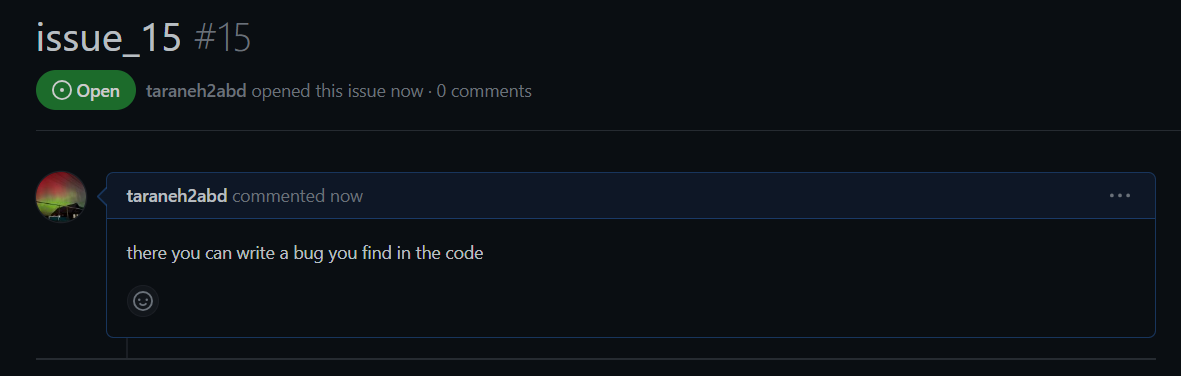
\includegraphics[width=1\textwidth]{issues.png}
    \caption{Screenshot depicting repository issues.}
\end{figure}

\end{document}
